\documentclass[11pt]{article}
\usepackage[a4paper,margin=1in]{geometry}
\usepackage[T1]{fontenc}
\usepackage[utf8]{inputenc}
\usepackage{lmodern}
\usepackage{hyperref}
\usepackage{enumitem}
\usepackage{booktabs}
\usepackage{graphicx}
\usepackage{float}
\usepackage{placeins}
\usepackage{tabularx}
\usepackage{xcolor}

\graphicspath{{../diagrams/}}

\hypersetup{
  colorlinks=true,
  linkcolor=blue,
  urlcolor=blue,
  pdftitle={Cloud Computing Project Plan - Hire Lens}
}

\title{Cloud Computing Project Plan\\\large Hire Lens}
\author{Mohammed Zaid Shaikh \and Piotr Bartosiewicz \and Krzysztof Krawiec}
\date{April 2026}

\begin{document}
\maketitle
\tableofcontents
\newpage

\section{Brief Description}
We propose a Telegram-first cloud platform that helps HR teams analyze GitHub profiles of candidates and compare them against job descriptions. The bot will generate a structured profile review from a GitHub username or profile URL, summarize public activity, highlight technical strengths and weak signals, and later support linked profiles such as GitHub, LinkedIn, and personal websites.

The first version focuses on safe, explainable automation: the bot will retrieve public GitHub information, run scoring and summarization workflows, and present a concise report to the HR user. In later iterations, the system can include AI-assisted compatibility scoring between a candidate profile and a job description.

A small web dashboard may be added later for admin and analytics tasks, but the Telegram bot remains the primary frontend.

To avoid dependence on paid AI APIs, the analysis layer can be powered by a self-hosted open-source model such as Qwen. The model would run behind an internal inference service and be called only by our backend, which keeps prompts, data, and costs under our control.

\subsection{Recommended Hosting Choice}
The easiest beginner-friendly hosting setup on Azure is:
\begin{itemize}[leftmargin=*]
  \item \textbf{Azure Functions}: Telegram webhook, OAuth callbacks, report endpoints, and access-control logic.
  \item \textbf{Azure Container Apps}: the self-hosted model-inference service, exposed only internally to the backend.
  \item \textbf{Azure Static Web Apps}: a small admin dashboard if we need one.
  \item \textbf{Azure Cosmos DB, Blob Storage, and Service Bus}: managed data, files, and background jobs.
\end{itemize}

This avoids AKS, avoids always-on virtual machines for the application layer, and keeps the infra simple enough for beginners while still being realistic for the course.

\section{Main Features}
\begin{enumerate}[leftmargin=*]
  \item \textbf{Telegram profile review}: HR sends a GitHub username or link and gets a structured evaluation.
  \item \textbf{Job description comparison}: HR can paste a job description and receive a compatibility summary.
  \item \textbf{Candidate shortlisting}: save candidate reports, tags, and follow-up notes.
  \item \textbf{Public-data enrichment}: gather public GitHub signals such as repositories, languages, commits, followers, stars, and contribution patterns.
  \item \textbf{Access control}: limit usage by subscription tier and organization role.
  \item \textbf{Notification scheduling}: send reminders, report updates, and saved-search alerts.
  \item \textbf{Payment readiness}: Stripe can be added later for premium access plans.
\end{enumerate}

\section{Typical User Roles}
\begin{itemize}[leftmargin=*]
  \item \textbf{HR Recruiter}: searches and reviews candidates, compares profiles with job descriptions, and saves reports.
  \item \textbf{Team Lead/Manager}: reviews shortlisted candidates and monitors report quality.
  \item \textbf{Platform Admin}: manages user access, usage limits, and billing tiers.
\end{itemize}

\section{System Architecture}
\subsection{Service Overview}
\begin{itemize}[leftmargin=*]
  \item \textbf{Frontend}: Telegram bot as the primary UI.
  \item \textbf{Optional Admin UI}: lightweight React dashboard for analytics and moderation.
  \item \textbf{API Layer}: Azure Functions exposing REST endpoints for bot actions and admin operations.
  \item \textbf{Auth}: Google/Facebook sign-in through OAuth, with no password storage.
  \item \textbf{Session Layer}: server-side session or short-lived token session store.
  \item \textbf{Primary Data}: Azure Cosmos DB for users, candidate reports, access rules, and usage records.
  \item \textbf{Unstructured Assets}: Azure Blob Storage for report exports, cached snapshots, and attachments.
  \item \textbf{Async Work}: Azure Service Bus and scheduled Functions for profile refresh, notifications, and ranking jobs.
  \item \textbf{Observability}: Application Insights and Azure Monitor with alerts.
\end{itemize}

\subsection{Microservice-style Functions}
\begin{itemize}[leftmargin=*]
  \item \texttt{bot-gateway-service}: receives Telegram updates and routes commands.
  \item \texttt{auth-service}: handles OAuth sign-in, session creation, and access checks.
  \item \texttt{profile-analysis-service}: fetches public GitHub data and creates profile summaries.
  \item \texttt{model-inference-service}: runs a self-hosted open-source model such as Qwen inside Azure Container Apps.
  \item \texttt{job-match-service}: compares candidate profiles with job descriptions using rule-based logic plus model output.
  \item \texttt{report-service}: stores and retrieves analysis reports.
  \item \texttt{notification-service}: scheduled reminders and saved-search alerts.
  \item \texttt{billing-service}: premium plan logic and Stripe integration for later versions.
\end{itemize}

\section{API Design}
Representative REST endpoints:
\begin{itemize}[leftmargin=*]
  \item \texttt{POST /api/v1/auth/oauth/start}
  \item \texttt{POST /api/v1/auth/oauth/callback}
  \item \texttt{POST /api/v1/bot/webhook}
  \item \texttt{POST /api/v1/profiles/analyze}
  \item \texttt{POST /api/v1/models/infer}
  \item \texttt{POST /api/v1/match/compare}
  \item \texttt{GET /api/v1/reports/{reportId}}
  \item \texttt{GET /api/v1/users/me/usage}
  \item \texttt{POST /api/v1/admin/limits}
\end{itemize}

\section{Storage Characteristics}
\begin{table}[ht!]
\centering
\small
\begin{tabularx}{\textwidth}{p{2.8cm}X p{2.2cm}X X}
\toprule
\textbf{Store} & \textbf{Type} & \textbf{Consistency} & \textbf{RW Pattern} & \textbf{Data Scope} \\
\midrule
Azure Cosmos DB & NoSQL, semi-structured documents & Tunable consistency, strong for critical records & Heavy read/write & Users, sessions, reports, usage limits, billing flags \\
Azure Blob Storage & Unstructured objects & Strong read-after-write for object access & Read-heavy with periodic writes & Report exports, cached payloads, attachments \\
Azure Table Storage or SQL (optional) & Structured metadata & Strong for transactional data, depending on choice & Moderate read/write & Audit logs, subscriptions, premium access records \\
\bottomrule
\end{tabularx}
\caption{Planned storage profile and access patterns.}
\end{table}

\section{Terraform Plan}
Infrastructure will be provisioned with Terraform and kept reproducible from the beginning:
\begin{itemize}[leftmargin=*]
  \item \texttt{modules/frontend} for Azure Static Web Apps and the optional dashboard deployment.
  \item \texttt{modules/functions} for Azure Functions, Telegram webhooks, OAuth callbacks, and scheduled jobs.
  \item \texttt{modules/auth} for OAuth and session-related resources.
  \item \texttt{modules/data} for Cosmos DB, Blob Storage, and optional SQL/Table resources.
  \item \texttt{modules/messaging} for Service Bus queues and topics.
  \item \texttt{modules/model} for Azure Container Apps hosting the self-hosted inference service.
  \item \texttt{modules/monitoring} for dashboards and alerting.
  \item \texttt{environments/dev} and \texttt{environments/prod} for environment-specific variables.
\end{itemize}

\noindent Minimum deliverable: one \texttt{terraform apply} that creates a working dev environment with bot backend, internal model service, database, storage, async messaging, and monitoring.

\section{Diagrams}
The following diagrams are included in the submission package.

\subsection{Architecture Diagram}
\begin{figure}[H]
\centering
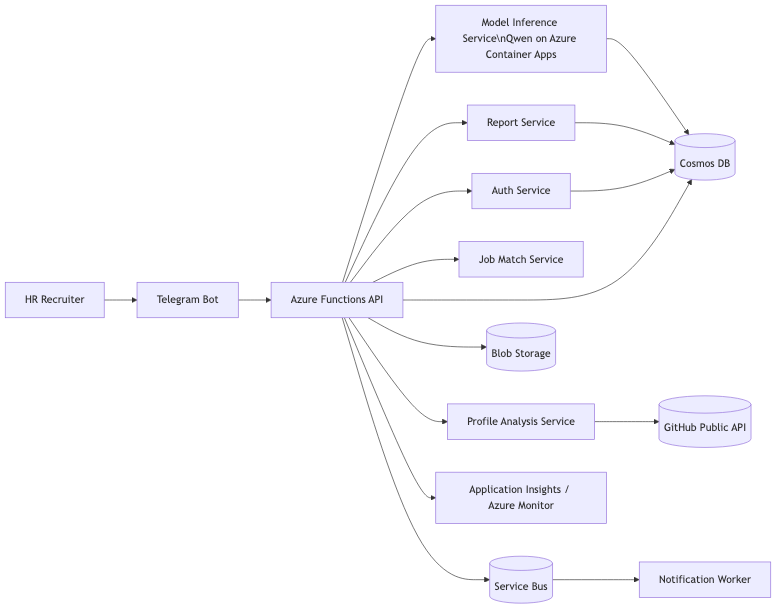
\includegraphics[width=\textwidth]{architecture.png}
\caption{System architecture diagram.}
\end{figure}

\subsection{Request Flow Diagram}
\begin{figure}[H]
\centering
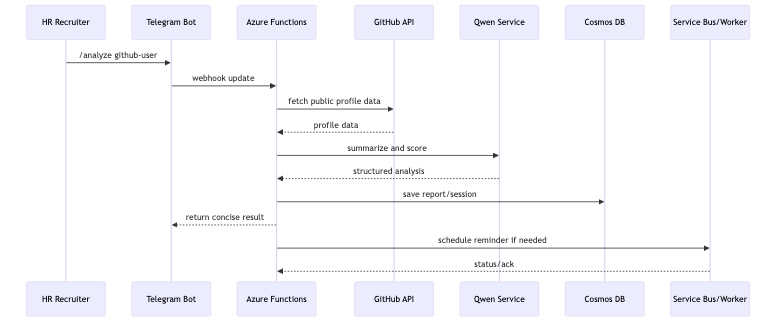
\includegraphics[width=\textwidth]{request-flow.png}
\caption{Request flow diagram.}
\end{figure}

\subsection{Storage Diagram}
\begin{figure}[H]
\centering
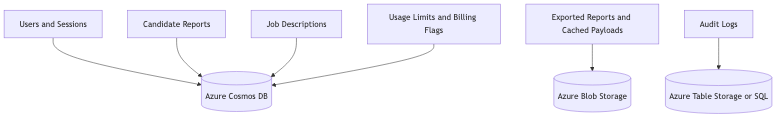
\includegraphics[width=0.9\textwidth]{storage.png}
\caption{Storage layout diagram.}
\end{figure}

\FloatBarrier

\section{Large-Scale Assumption}
The architecture assumes thousands of HR users and repeated candidate reviews per day, with spikes during hiring campaigns. Scaling strategy:
\begin{itemize}[leftmargin=*]
  \item Stateless Azure Functions that scale on demand.
  \item Queue-based processing for profile analysis and enrichment jobs.
  \item Azure Container Apps for the model endpoint so inference cost is predictable and data stays inside our system.
  \item Caching of frequent GitHub responses and report snapshots.
  \item Rate limiting and access tiers to protect public API usage and cloud costs.
\end{itemize}


\section{Service Level Agreement (SLA)}

This Service Level Agreement defines the expected reliability, performance, and operational guarantees of the Hire Lens platform deployed in a cloud environment.

\subsection{Service Scope}
The SLA applies to the following system components:
\begin{itemize}[leftmargin=*]
  \item Telegram bot interaction layer (bot-gateway-service)
  \item Backend API (Azure Functions)
  \item Profile analysis and job matching services
  \item Internal model inference service
  \item Data storage (Cosmos DB, Blob Storage)
\end{itemize}

External dependencies such as GitHub API and OAuth providers are excluded from strict guarantees but are considered in best-effort availability.

\subsection{Service Level Indicator (SLI)}
A Service Level Indicator we defined as the percentage of successful HTTP requests relative to the total number of HTTP requests over a specified time period. A request is considered successful if it returns a response with status code 200-399 within the acceptable response time.

\subsection{Service Level Objectives (SLO)}

The system defines the following Service Level Objectives based on the SLI metrics:

\begin{itemize}[leftmargin=*]
  \item \textbf{Availability SLO:} 99.0\% of requests are successful over a monthly period
  \item \textbf{Latency SLO:} 95\% of requests are served within 2 seconds
  \item \textbf{Error Rate SLO:} less than 1\% of requests result in errors (HTTP 5xx or timeout)
\end{itemize}

\subsection{Performance (Latency Objectives)}
The system defines the following response time objectives:

\begin{itemize}[leftmargin=*]
  \item \textbf{API response time:} below 2 seconds
  \item \textbf{Maximum response time:} 5 seconds
  \item \textbf{Model inference response time:} below 2 minutes (asynchronous processing allowed)
\end{itemize}

Long-running operations such as profile analysis may be processed asynchronously using queues.


\subsection{Error Rate}
\begin{itemize}[leftmargin=*]
  \item \textbf{Target error rate:} less than 1\% of total requests
  \item Errors include HTTP 5xx responses and timeouts
\end{itemize}

\subsection{Security}
\begin{itemize}[leftmargin=*]
  \item All communication is secured via HTTPS
  \item OAuth-based authentication (no password storage)
  \item Access control enforced per user role and subscription tier
\end{itemize}

\subsection{Monitoring and Observability}
The system uses cloud-native monitoring tools:
\begin{itemize}[leftmargin=*]
  \item Azure Monitor and Application Insights for logs and metrics
  \item Alerting on:
  \begin{itemize}
    \item high error rate
    \item increased latency
    \item service downtime
  \end{itemize}
\end{itemize}

\subsection{Maintenance and Downtime}
\begin{itemize}[leftmargin=*]
  \item Planned maintenance will be scheduled during low-traffic periods
  \item Users will be notified in advance when possible
  \item Planned downtime is excluded from SLA calculations
\end{itemize}


\subsection{Violation Handling}
In case the SLA objectives are not met:
\begin{itemize}[leftmargin=*]
  \item The incident is recorded and analyzed
  \item Root cause analysis is performed
  \item Improvements are proposed for future iterations
\end{itemize}


\section{Delivery Plan and Team Split}
\subsection{Submission Scope}
\begin{itemize}[leftmargin=*]
  \item Final project idea, features, user roles, and high-level architecture.
  \item Diagram sources in Mermaid format for the final submission package.
  \item API design, storage profile, Terraform setup, and SLA/SLO/SLI definitions.
  \item Live-demo plan with AI-assisted comparison and usage limits.
\end{itemize}

\subsection{Proposed Responsibilities}
\begin{itemize}[leftmargin=*]
  \item \textbf{Mohammed Zaid Shaikh}: Telegram bot flow, UX, and command handling.
  \item \textbf{Piotr Bartosiewicz}: Azure Functions, GitHub analysis logic, and API contracts.
  \item \textbf{Krzysztof Krawiec}: Terraform, monitoring, deployment automation, and load testing.
\end{itemize}

\section{Risk and Mitigation}
\begin{itemize}[leftmargin=*]
  \item \textbf{Risk}: GitHub public API rate limits.
  \item \textbf{Mitigation}: caching, queueing, and conservative refresh intervals.
  \item \textbf{Risk}: AI output quality or hallucination.
  \item \textbf{Mitigation}: structured prompts, explainable scoring, and fallback rule-based summaries.
  \item \textbf{Risk}: GPU hosting cost for the open-source model.
  \item \textbf{Mitigation}: start with a smaller quantized Qwen model on Azure Container Apps, keep inference behind caching and rate limits, and move to a GPU-only option only if performance is not enough.
  \item \textbf{Risk}: OAuth setup complexity for beginners.
  \item \textbf{Mitigation}: start with one provider, then add the second provider once the flow is stable.
  \item \textbf{Risk}: Costs increase with external API calls and network traffic.
  \item \textbf{Mitigation}: use the cheapest practical Azure region, limit retries, and add usage caps per tier.
\end{itemize}

\section{Conclusion}
This project keeps the implementation practical while still looking like a serious cloud system: a Telegram-first product, Azure managed services, Terraform-based infrastructure, and a clear path from rule-based analysis to AI-assisted hiring support.

\end{document}
